\section{Demonstrator Prototype}
\label{sec:design}

About 4 pages on:

\begin{enumerate}

\item An architectural overview of the application that has been implemented
\item High-level design, domain model, … (App assignment A)
\item May involve selected models from Chaps. 5 of the IoT and cloud books


\end{enumerate}

To get an overview of how we wanted to implement the user interface, an application flow diagram was modeled. 
The diagram displays how the user navigates through the different frames in the front end of the application:
\begin{figure}
  \centering
  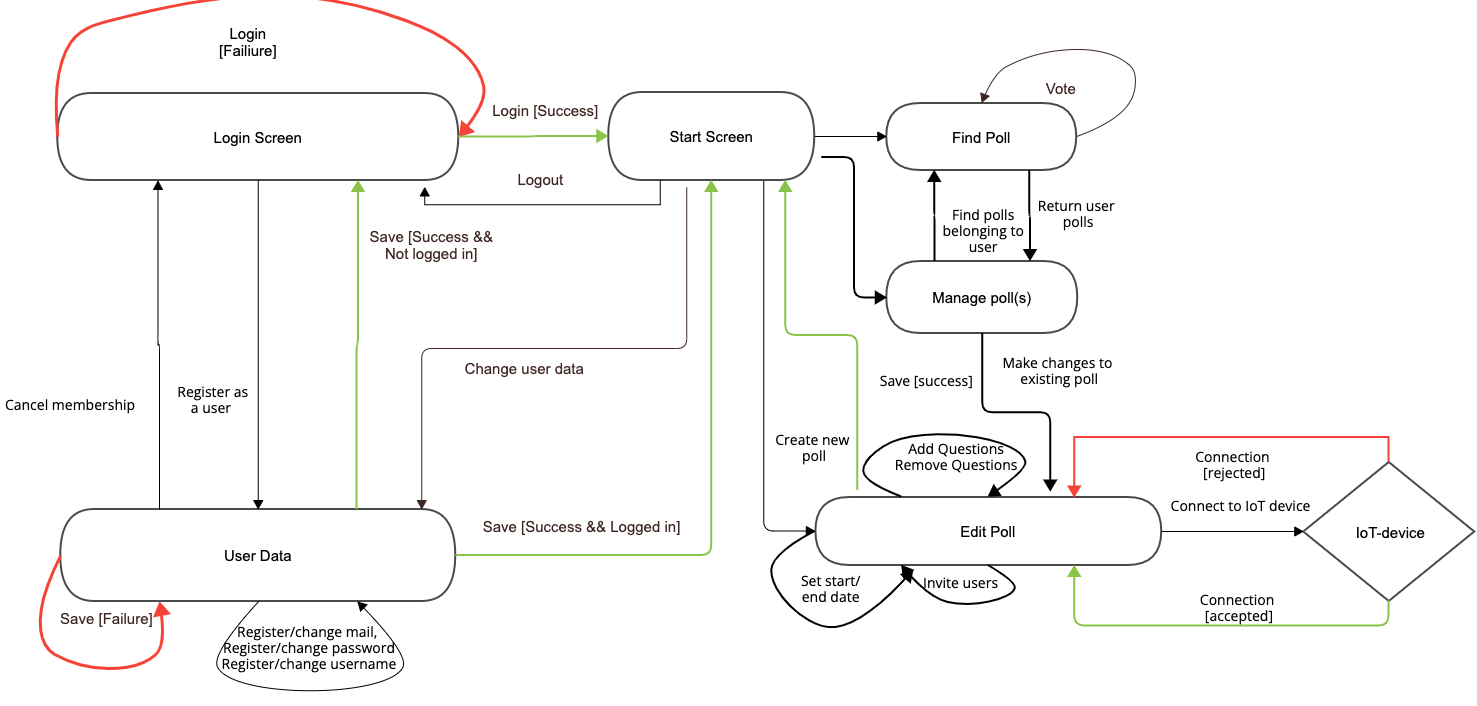
\includegraphics[scale=0.30]{figs/Application Flow Diagram (1).png}
  \caption{Application Flow Diagram}
  \label{fig:appFlow}
\end{figure}

Each screen has in the diagram been modelled as a state, and for every state, the user is able to do some action or provide some input. 
These actions or inputs are modelled as transitions, and are in the figure above illustrated with arrows. Transitions that results in errors are 
colored red, and transitions that does not result in errors are colored green. Our application consists of six screens. We have a login screen, 
where the user can either login, or create a new user. Once the user is logged in, he is directed to a start screen, where he gets the option to 
do multiple actions. He can search for a poll, which then can be voted on, or he can view and manage his own polls. He can create new polls,
and in this state he gets the option to pair the poll with an IoT device. 

The example below shows how you may include code. There are similar
styles for many other langages - in case you do not use Java in your
project. You can wrap the listing into a figure in case you need to
refer to it. How to create a figure was shown in Section~\ref{sec:technology}.

\lstinputlisting[language=java]{code/BoksVolum.java}
